\documentclass[12pt]{article}
\usepackage{graphicx}
\usepackage{fullpage}
\usepackage{float}
\title{Predicting Region of Origin of Indian Dishes with Naive Bayes Text Classification}
\author{Audrey Shingleton}

\begin{document}
\maketitle

\section{Introduction}
The food we eat around the world is often a reflection of the culture of its origin. People can typically recognize that a noodle dish featuring soy sauce and ginger (common ingredients of chow mein) is from China whereas noodles with marinara and parmesan is from Italy. This lead me to wonder if I could develop a machine learning method that, given information about a dish, could predict where that dish is from.\\ 


\noindent As it turns out, there is existing work that looks into this question. Sajadmanesh et al.\cite{Sajadmanesh} specifically addressed how good we can predict cuisine (country) given ingredients. Their Deep Neural Network classifier was able to achieve nearly a 75\% test set accuracy for predicting geographical region and found strong ingredient diversity across continents.
Min et al.\cite{Min} used textual and visual information to summarize differences in cuisine. This was done with a Bayesian Cuisine-Course Topic Model (BC\textsuperscript{2}TM) which breaks up a recipe into common and cuisine-specific ingredients. A manifold ranking method was then used to select food images for the groups found from the BC\textsuperscript{2}TM. Their methods were able to categorize ingredients based on cusisine type. \\

\noindent While both of these papers show very promising results in the ability to predict cuisine across countries and continents, they do not examine the subtleties found in intra-country culture. For instance, just within the United States, the hoppin' John rice dish has history in the South and American goulash is recognized as belonging to the Midwest.
It seems like methods exist that could determine that both of these dishes are American food, but could a machine learning algorithm predict their region of origin within the U.S.? This may be a more difficult task as the differences in these dishes is less drastic than the chow mein vs. spaghetti example. Essentially, I expect culture differences within a country to be less recognizable than culture differences between countries.\\

\noindent I have found a dataset from Kaggle of Indian food (https://www.kaggle.com/nehaprabhavalkar/indian-food-101) that gives information about a dish and its region of origin. Indian cuisine consists of a variety of regional and traditional dishes. Given the diversity in soil, climate, culture, ethnic groups, occupations, and religion, dishes can vary substantially across the country. My project will aim to predict the region of a dish within India based on recipe information using Naive Bayes classification. 

\section{Methods}
\subsection{Data}
The initial datasetset consisted of 255 unique recipes with 8 features: ingredients, diet, prep time, cook time, flavor profile, course, state, and region. 
All data is text information aside from prep time and cook time which are numeric.
The classification will be done with 6 geographical regions (within India) which are Central, East, North, North East, South, and West. 
I will be ignoring the dish name and state attributes in the dataset as the dish name acts as a unique ID for each recipe and the state would directly provide information about 
the region.
After removing data with missing features, I was left with 242 recipe items where 193 (80\%)
will be used for training and the remaining 49 for testing.

\subsection{Initial Model}

\noindent I hypothesized that the ingredients of a dish would be the best representation of its culture (as in Sajadmanesh et al.\cite{Sajadmanesh}). Thus, The aim of my initial classifier was to predict region of origin with just the ingredients of a dish.
As the ingredients are a list of text data, I decided to use Multinomial Naive Bayes (MNB) classification. \\

\noindent MNB is best suited for discrete data like word counts, as seen with the classic ham/spam e-mail classification problem. It is a way to model the distribution of words in a document as a multinomial\cite{Rennie}. For my particular problem, this is the distribution of ingredients in an Indian dish. Each dish is treated as a sequence of words where it is assumed that the word position is independent of the others. With a fixed number of regions for classification, the parameter vector for a class $c$ is $\vec{\theta_c} = \{\theta_{c1}, \theta_{c2}, ..., \theta_{cn} \}$ where $n$ is the size of the vocabulary. Using an estimate of the prior distribution over the regions $p(\vec{\theta_c})$, we can perfrom classification by selecting the region with the largest posterior probability. The MNB classifier is then defined as
\begin{center}
$l(d) = argmax_c [log(p(\vec{\theta_c})) + \sum_{w} f_w log(\theta_{cw})]$
\end{center}
where $f_w$ is the frequency count of each word $w$ in dish $d$.
The output $l(d)$ will be the predicted class of dish $d$. \\
 
\noindent The multinomial parameter $\vec{\theta_{cw}}$ is estimated as the number of times a word $w$ appears in the dishes of class $c$ $(N_{cw})$, divided by the total number of words in that class ($N_c$).
For each word $w$, the value $\alpha_w$ is added to its occurrences so that the estimates will never have a probability of zero. I set $\alpha_w = 1$ to follow common practice. I then substituted the parameter estimate
\begin{center}
$\hat{\theta}_{cw} = \frac{N_{cw} + \alpha_w}{N_c + \alpha}$
\end{center}
for the true parameter $\theta_{cw}$, where $\alpha$ is the sum of $\alpha_w$.

\subsection{Model Revision: Additional Features}

\noindent As my initial model only used one feature from the dataset (ingredients), I revised my classifier to include diet, prep time, cook time, flavor profile, and course. As both prep time and cook time were numeric features, I discretized them into categories. This lead to the question of how to best discretize these features for optimal classification. Yang et al.\cite{Yang} analyzed various discretization methods specifically for Naive Bayes classification.
They found that the weighted proportional k-Interval discretization (WPKID), an improved version of proportional k-Interval discretization (PKID), is best for smaller datasets, where fewer intervals with more instances may be best. WKPID weighs discretization such that, as traning data size $n_{train}$ increases, so does both the interval size $s$ above a set minimum and the number of intervals $t$. This minimum interval size $m$ is typically set to 30 as it is generally the minimum sample from which one should draw statistical inferences \cite{Yang}. The interval length and number of intervals is calculated as
\begin{center}
$s \cdot t = n_{train}$ \\
$s - m = t$ \\
$m = 30$ \\
\end{center}

\noindent Because my training data was on the smaller side with 193 instances, the WKPID method looked like the best method to use for my problem. Given $m = 30$ and $n_{train} = 193$, the interval size and number of intervals were 35 and 5 respectively. After discretization, I mapped the prep time and cook time to their corresponding interval labels. They could then be treated as text data to easily flow into my MNB implementation.

\subsection{Model Revision: Complement Naive Bayes}
When developing my initial model, I noticed that my training data was unbalanced in the number of instances per region. Specifically, the number of data instances were 2, 24, 42, 19, 46, and 60 for Central, East, North, North East, South, and West respectively. 

\noindent In previous work by Rennie et al.\cite{Rennie}, it was found that skewed data (having unbalanced training examples for each class) can create problems for Naive Bayes text classifiers. This is because it can cause the classifier to unintentionally prefer a certain class over the other.
To deal with this, they proposed using Complement Naive Bayes (CNB) classification.
While MNB estimates weights using data from a single class $c$, CNB estimates weights with a complement class. The complement class uses information from every class except $c$, which will be represented as $\hat{c}$, such that more data will be used per parameter estimate to mitigate data bias \cite{Rennie}.
The complement parameter estimate is
\begin{center}
$\hat{\theta}_{\hat{c}w} = \frac{N_{\hat{c}w} + \alpha_w}{N_{\hat{c}} + \alpha}$
\end{center}
where $N_{\hat{c}w}$ is the number of times word $w$ occurred in classes except $c$ and $N_{\hat{c}}$ is
the total number of words in classes except $c$.
The CNB classifier is then defined as
\begin{center}
$l(d) = argmax_c [log(p(\vec{\theta_c})) - \sum_{w} f_w log(\frac{N_{\hat{c}w} + \alpha_w}{N_{\hat{c}} + \alpha})]$
\end{center}
where the negative sign shows that we classify documents to class $c$ if they poorly match the complement parameter estimates.

\section{Results}
After estimating the parameters for each of my classifiers (described in sections 2.2-2.4) with the training data, I evaluated their performance by comparing the predicted region with the true region for each dish in the test set.\\\

\noindent Results from the MNB classifier with ingredients only:\\
\begin{table}[H]
   \centering
\begin{tabular}{ |c| } 
 \hline
 Training set accuracy: 87.05\% \\ 
 \hline
 Test set accuracy: 55.10\% \\ 
 \hline
\end{tabular}
\caption{MNB accuracy}
\label{table:mnb}
\end{table}

\begin{figure}[H]
   \centering
   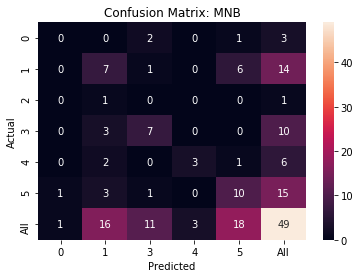
\includegraphics{mnb.png}
   \caption{MNB confusion matrix}
   \label{fig:mnb}
\end{figure}

\noindent Table \ref{table:mnb} shows that the initial MNB classifier performed really well on the training set but lost over 30\% accuray on the test set, dropping to 55\%. As shown in Figure \ref{fig:mnb}, region 3 had the best prediction accuracy of 70\% (7 predicted / 10 actual). Region 5 was not far behind with 66\% accuracy, and regions 1 and 3 both had 50\%. Regions 0 and 2 had the lowest accuracy with 0\%. In fact, none of the dishes were predicted as being from region 2.\\


\noindent Results from the MNB classifier with additional dish features:\\
\begin{table}[H]
   \centering
\begin{tabular}{ |c| } 
 \hline
 Training set accuracy: 81.87\% \\ 
 \hline
 Test set accuracy: 57.15\% \\ 
 \hline
\end{tabular}
\caption{MNB revised accuracy}
\label{table:mnb2}
\end{table}

\begin{figure}[H]
   \centering
   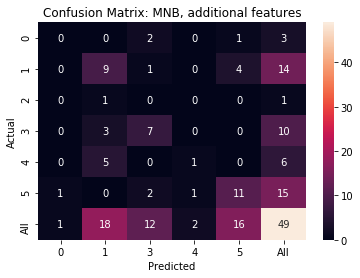
\includegraphics{mnb2.png}
      \caption{MNB revised confusion matrix}
   \label{fig:mnb2}
\end{figure}

\noindent The MNB classifer using additional dish features performed just slightly better than before (Table \ref{table:mnb2}). There was still a decently large gap between training and test set accuracy. From Figure \ref{fig:mnb2}, we can see that this classifier performed the best with region 5 with 73\% accuracy. As compared to Figure \ref{fig:mnb}, region 3 remained at 70\% accuracy and region 1 got a small improvement moving up to 64\%. There was also fairly dramatic decrease for region 4 going from 50\% down to 16\%. Regions 0 and 2 still had 0\% accuracy, with no dishes predicted as being from region 2.\\

\noindent Results from the CNB classifier:\\
\begin{table}[H]
   \centering
\begin{tabular}{ |c| } 
 \hline
 Training set accuracy: 67.36\% \\ 
 \hline
 Test set accuracy: 53.06\% \\ 
 \hline
\end{tabular}
\caption{CNB accuracy}
\label{table:cnb}
\end{table}

\begin{figure}[H]
   \centering
   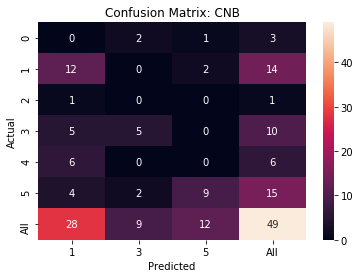
\includegraphics{cnb.png}
   \caption{CNB confusion matrix}
   \label{fig:cnb}
\end{figure}

\noindent Table \ref{table:cnb} shows that CNB classification had the lowest test set accuracy as compared to the other classifiers. However, the difference between its training and test set accuracy was much smaller (about 15\%). From Figure \ref{fig:cnb}, CNB classification performed really well for class 1 with 85.7\% accuracy. However, there were decreases in accuracy for all other regions as compared to Figures \ref{fig:mnb} and \ref{fig:mnb2}. No dishes were predicted as being from regions 0, 2, and 4.

\section{Discussion}

\noindent All of my classifiers performed better than random (16.67\%) and were all within 5\% test set accuracy of each other. CNB classification performed the worst with 53\% test set accuracy and MNB (using only ingredients) was the best with 57\%. Due to the fact that the test set only had 49 data instances, this difference only equates to two data misclassifications. Therefore, all classifiers were fairly equivalent in performance.\\

\noindent The additional dish features used in my revised MNB classifier did not prove to be useful as it only lead to a measly 2\% improvement in test set accuracy. This shows that the ingredients of a dish most likely gives the most information on the culture of its region of origin.\\

\noindent I also noted that the training set accuracy was much greater than the test set for both MNB classifiers. This signals that there may have been overfitting that didn't allow the classifier to pick up on more general patterns in the data. For the CNB classifier, the training set accuracy was not much larger than the test set. This shows that CNB may be the best at not overfitting to the training data.
As CNB did not predict any dishes as belonging to regions 0, 2, and 4 (North East, Central, and East), this could show that these regions did not have strong patterns in their dish features.\\

\noindent It was interesting that region 5, which is the South, had the one of the highest (or the highest) prediction accuracy for all classifiers. This shows that Southern Indian cuisine may be the most distinct compared to the other regions. Regions 1 and 3, the West and North, also had decent classification accuracy, ranging from 50\% to 85\%. From these results, we can hypothesize that the South, West, and North have the most distinct culture in India or that they have greatly influenced the other regions such that most examples are classified as belonging to one of them.\\

\section{Conclusion}

\noindent I examined the use of MNB and CNB text classification to predict the region of origin within India given information about a dish. While prior work was able to pick out differences in cuisine between countries \cite{Min, Sajadmanesh}, it was much more difficult to recognize cuisine differences within a country as both classifiers could only achieve 53-57\% accuracy on predicting the correct region of the test data. These results may help to highlight the cultural differences and similarities between the regions of India, a country rich in diversity and full of history, showcased by their unique cuisine. Additionally, this analysis may help to highlight the difficulties in intra-country cuisine classification where dish differences are not as easily recognized as they are when comparing dishes from different countries.

\section{Works Cited}
\begin{thebibliography}{9}
\bibitem{Min} 
Min, Weiqing, et al. “You Are What You Eat: Exploring Rich Recipe Information for Cross-Region Food Analysis.” IEEE Transactions on Multimedia, vol. 20, no. 4, 2018, pp. 950–964.

\bibitem{Rennie} 
Rennie, Jason D., et al. "Tackling the poor assumptions of naive bayes text classifiers." Proceedings of the 20th international conference on machine learning (ICML-03). 2003.

\bibitem{Sajadmanesh}
Sajadmanesh, Sina, et al. “Kissing Cuisines.” Proceedings of the 26th International Conference on World Wide Web Companion - WWW '17 Companion, 2017, pp. 1013–1021.

\bibitem{Yang} 
Yang, Ying and Webb, Geoffrey I. "A Comparative Study of Discretization Methods for Naïve-Bayes Classifiers." Proceedings of PKAW 2002, The 2002 Pacific Rim Knowledge Acquisition Workshop, Tokyo, Japan.
\end{thebibliography}

\end{document}